\chapter{Results}
\label{ch:chapter_4}

%% The following annotation is customary for chapter which have already been
%% published as a paper.
%\blfootnote{Parts of this chapter have been published in Annalen der Physik \textbf{324}, 289 (1906) \cite{Einstein1906}.}

%% It is only necessary to list the authors if multiple people contributed
%% significantly to the chapter.
%\authors{Albert {\titleshape Einstein}}

%% The '0pt' option ensures that no extra vertical space follows this epigraph,
%% since there is another epigraph after it.
%\epigraph[0pt]{
%    "quote1"
%}{attribution}

\epigraph{
    “No amount of experimentation can ever prove me right;
    
    a single experiment can prove me wrong. ”
}{Albert Einstein}

\begin{abstract}
Is this abstract enough?
\end{abstract}

%% Start the actual chapter on a new page.
\newpage
\section{Introduction}
While I have found the rather elegant many-body Green's Function (equation~\ref{eq:mbgfresult}), this does not tell us what the exact predictions are as they largely depend on the particular system or molecule.

In \citet{perrinnano}, the authors found a pronounced Negative-Differential Conductance (NDC) which is readily explained from a two site model, which I present here. Note that while the NDC was qualitatively explained by the two-site model, they used a prefactor $7.2 \times 10^{-5}$ to match the absolute values of the current. This has yet to be explained, and the Coulomb interaction was our prime suspect.

In section~\ref{sec:twosite}, I define the model both with and without spin. I then move on to look at the transmission functions in section~\ref{sec:twositetransmission}. The $I(V)$ characteristics for selected parameter sweeps are presented in section~\ref{sec:twositeparamsweep}. Finally, the improvement on quantitative agreement with the experiment of Ref.~\cite{perrinnano} is shown in section~\ref{sec:perrin}.


\section{Two site model} 
\label{sec:twosite}
\subsection{Spinless two site model}
The form of the two-site model including Stark effect has been confirmed with DFT calculations in the supplement of Ref.~\cite{perrinnano}. I  will first look at the model without including spin. The Hamiltonian including tunnelling terms is:
\begin{align}
H_1 &= \begin{bmatrix} \epsilon_0 + \frac{1}{2} \alpha V & -\tau \\
-\tau & \epsilon_0 - \frac{1}{2} \alpha V\end{bmatrix},
\label{eq:spinlesshamiltonian}
\end{align}
where $\epsilon_0$ is the zero-bias level, $\tau$ is the tunnelling strength, $\alpha$ is the bias-level coupling due to the Stark effect and $V$ is the bias Voltage (in eV). The molecule is assumed to couple symmetrically to the left and right leads in the WBL:
\begin{align*}
\Gamma^L &= \begin{bmatrix} \Gamma & 0 \\ 0 & 0 \end{bmatrix},\\ \Gamma^R &= \begin{bmatrix} 0 & 0 \\ 0 & \Gamma \end{bmatrix},
\end{align*}
where $\Gamma$ is the molecule-lead coupling strength. The capacitive self-energy (equation~\ref{eq:selfenergycapacitive}) is given by:
\begin{align*}
\Sigma^c &= \begin{bmatrix} U & 0 \\ 0 & 0 \end{bmatrix} n_2 + \begin{bmatrix} 0 & 0 \\ 0 & U \end{bmatrix} n_1,
\end{align*}
where $U$ is the capacitive interaction strength.  The model is depicted schematically in figure~\ref{fig:twosite}, where I have explicitly drawn the capacitive interaction. The leads are at different heights due to applied bias.


\begin{figure}[!bt]
    \begin{subfigure}[b]{0.48\textwidth}
        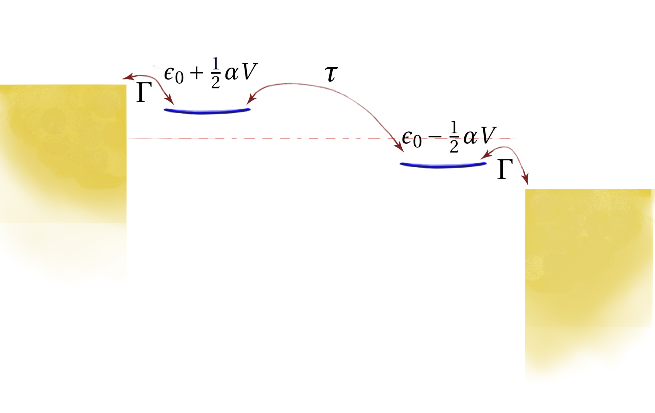
\includegraphics[height=.20\textheight]{pdf/non_interacting_schematics.pdf}\caption{Non-interacting}\label{fig:twositea}
    \end{subfigure}
    ~
    \begin{subfigure}[b]{0.48\textwidth}
        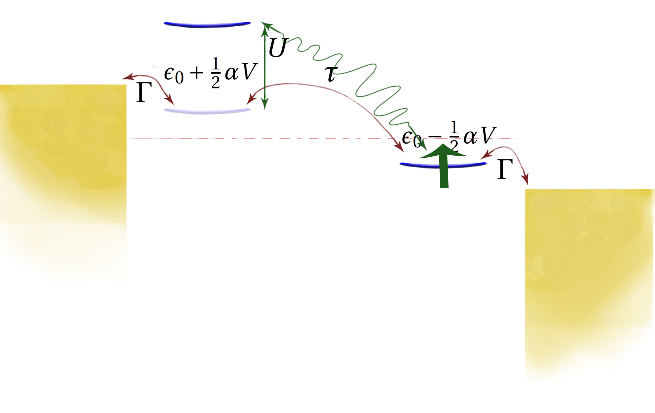
\includegraphics[height=.20\textheight]{pdf/interacting_schematics.pdf}\caption{Interacting}\label{fig:twositeb}
    \end{subfigure}
    \caption{Schematic pictures of the spinless two site model. The red dashed line denotes the Fermi-level. Figure~\ref{fig:twositea} shows the non-interacting case, where $\Gamma$ is the molecule-lead coupling, $\epsilon \pm \frac{1}{2} \alpha V$ are the left (right) level and $\tau$ is the tunnelling strength between the levels. In Figure~\ref{fig:twositeb}, an electron (large green arrow) occupies the right level. The swirly line is meant to indicate an interaction with electrons on the left level, thereby raising the level with the capacitive interaction or charging energy $U$.} \label{fig:twosite}
\end{figure}

When no capacitive interaction is included (i.e. $U=0$), the common method (section~\ref{sec:synthesis}) can be applied to find the transmission analytically: \cite{perrinnano}\footnote{If the bias voltage is assumed to be distributed symmetrically over the leads, then the current can be found analytically as well. However, this serves no purpose in this discussion.}:
\begin{align*}
T(\epsilon) &= \frac{ (2\tau)^2 }{(\frac{\Gamma}{2})^2} \frac{(\frac{\Gamma}{2})^2}{(\epsilon-\epsilon_1)^2 + (\frac{\Gamma}{2})^2}\frac{(\frac{\Gamma}{2})^2}{(\epsilon-\epsilon_2)^2 + (\frac{\Gamma}{2})^2},
\end{align*}
where $\epsilon_{1,2} = \epsilon_0 \pm \frac{1}{2} \Delta$, where $\Delta$ is the level splitting in the presence of bias voltage given by $\Delta = \sqrt{ (\alpha V)^2+ 4\tau^2}$. 

For the two-site model including capacitive interactions, we assume that the chance a many-body state $\ket{\kappa}$ is occupied is proportional to the Boltzmann-factor $e^{ -\beta \braket{ \kappa\left| H \right| \kappa}} Z^{-1}$, where $Z$ is a normalisation constant and $H$ the full Hamiltonian including capacitive interactions.

It is illustrative for the application of the many-body Green's function (equation~\ref{eq:mbgfresult}) to consider the shapes of $G^{\lambda\pm}$. Their most important contribution in this context is simply the thermal average of the capacitive self-energy $\braket{\lambda\left|\Sigma^c\right|\lambda}$. The four $G^{\lambda\pm}$ are:
\begin{align*}
G^{\ket{00}\pm} &= \left[ \epsilon \begin{bmatrix} 1 & 0 \\ 0 & 1 \end{bmatrix} - \begin{bmatrix} \epsilon_0 + \frac{1}{2} \alpha V & -\tau \\
-\tau & \epsilon_0 - \frac{1}{2} \alpha V\end{bmatrix}  \pm \frac{\imath}{2} \begin{pmatrix} \Gamma & 0 \\ 0 & \Gamma \end{pmatrix} \right]^{-1}, \\
G^{\ket{10}\pm} &= \left[ \epsilon \begin{bmatrix} 1 & 0 \\ 0 & 1 \end{bmatrix} - \begin{bmatrix} \epsilon_0 + \frac{1}{2} \alpha V & -\tau \\
-\tau & \epsilon_0 - \frac{1}{2} \alpha V\end{bmatrix} - \begin{pmatrix} 0 & 0 \\ 0 & U \end{pmatrix} \pm \frac{\imath}{2} \begin{pmatrix} \Gamma & 0 \\ 0 & \Gamma \end{pmatrix} \right]^{-1}, \\
G^{\ket{01}\pm} &= \left[ \epsilon \begin{bmatrix} 1 & 0 \\ 0 & 1 \end{bmatrix} - \begin{bmatrix} \epsilon_0 + \frac{1}{2} \alpha V & -\tau \\
-\tau & \epsilon_0 - \frac{1}{2} \alpha V\end{bmatrix} - \begin{pmatrix} U & 0 \\ 0 & 0 \end{pmatrix} \pm \frac{\imath}{2} \begin{pmatrix} \Gamma & 0 \\ 0 & \Gamma \end{pmatrix} \right]^{-1},\\
G^{\ket{11}\pm} &= \left[ \epsilon \begin{bmatrix} 1 & 0 \\ 0 & 1 \end{bmatrix} - \begin{bmatrix} \epsilon_0 + \frac{1}{2} \alpha V & -\tau \\
-\tau & \epsilon_0 - \frac{1}{2} \alpha V\end{bmatrix} - \begin{pmatrix} U & 0 \\ 0 & U \end{pmatrix} \pm \frac{\imath}{2} \begin{pmatrix} \Gamma & 0 \\ 0 & \Gamma \end{pmatrix} \right]^{-1},
\end{align*}
where we see that adding an electron to e.g. $\ket{10}$ would add the energy $\epsilon_2$ and the capacitive interaction energy $U$. We see this quite clearly in the capacitive self-energy contribution of $G^{\ket{10}\pm}$. 

\subsection{Spinfull two site model}
When we include spin in the model, we are essentially keeping two copies of the model and add interaction. There is no spin-flip tunnelling. I use the ordered many-body basis $\left\{ \ket{\uparrow 1}, \ket{\downarrow 1}, \ket{\uparrow 2}, \ket{\downarrow 2}\right\}$. The Hamiltonian is:
\begin{align}
H_1 &= \begin{bmatrix} \epsilon_0 + \frac{1}{2} \alpha V & 0 & -\tau & 0 \\ 0 & \epsilon_0 + \frac{1}{2} \alpha V & 0 & -\tau\\ -\tau & 0 & \epsilon_0 - \frac{1}{2} \alpha V & 0 \\ 0 & -\tau & 0 & \epsilon_0 - \frac{1}{2} \alpha V\end{bmatrix},
\label{eq:spinfullhamiltonian}
\end{align} 
while the coupling matrices are:
\begin{align*}
\Gamma^L &= \begin{bmatrix} \Gamma & 0 & 0 & 0 \\ 0 & \Gamma & 0 & 0 \\ 0 & 0 & 0 & 0 \\  0 & 0 & 0 & 0\end{bmatrix},\\ \Gamma^R &= \begin{bmatrix} 0 & 0 & 0 & 0 \\ 0 & 0 & 0 & 0 \\ 0 & 0 & \Gamma & 0 \\ 0 & 0 & 0 & \Gamma \\ \end{bmatrix},
\end{align*}
and the capacitive self-energy is:
\begin{align*}
\Sigma^c &= \begin{bmatrix} \zeta U & 0 & 0 & 0\\ 0 & \zeta U & 0 & 0\\ 0 & 0 & 0 & 0\\ 0 & 0 & 0 & \xi U \end{bmatrix} n_{\uparrow 2} + \begin{bmatrix} \zeta U & 0 & 0 & 0\\ 0 & \zeta U & 0 & 0\\ 0 & 0 & \xi U & 0\\ 0 & 0 & 0 & 0 \end{bmatrix} n_{\downarrow 2} +\\
&\quad\begin{bmatrix} 0 & 0 & 0 & 0\\ 0 & \xi  U & 0 & 0\\ 0 & 0 & \zeta U & 0\\ 0 & 0 & 0 & \zeta U \end{bmatrix} n_{\uparrow 1} + \begin{bmatrix} \xi  U & 0 & 0 & 0\\ 0 & 0 & 0 & 0\\ 0 & 0 & \zeta U & 0\\ 0 & 0 & 0 & \zeta U \end{bmatrix} n_{\downarrow 1},
\end{align*}
where $\zeta U$ describes the strength of capacitive interaction between the left and right site (intersite), whereas $\xi U$ describes the strength of capacitive interaction on the left or right site (onsite).

\section{Transmission}
\label{sec:twositetransmission}
\section{Current parameter sweeps}
\label{sec:twositeparamsweep}
\section{Experimental fit}
\label{sec:perrin}
\references{dissertation}